\documentclass[conference]{IEEEtran}
\IEEEoverridecommandlockouts

\usepackage{cite}
\usepackage{amsmath,amssymb,amsfonts}
\usepackage{algorithmic}
\usepackage{graphicx}
\usepackage{textcomp}
\usepackage{xcolor}
\usepackage{booktabs}
\usepackage{multirow}
\usepackage{tikz}
\usetikzlibrary{shapes.geometric, arrows, positioning, fit, backgrounds}
\usepackage{pgfplots}
\pgfplotsset{compat=1.17}
\usepackage{hyperref}
\usepackage{cleveref}

\def\BibTeX{{\rm B\kern-.05em{\sc i\kern-.025em b}\kern-.08em
    T\kern-.1667em\lower.7ex\hbox{E}\kern-.125emX}}

\begin{document}

\title{Early Detection of Model Collapse in Large Language Models: A Diversity-Based Framework}

\author{\IEEEauthorblockN{Kamal Singh Bisht, \textit{Senior Member, IEEE}}
\IEEEauthorblockA{Independent Researcher\\
Frisco, Texas, USA\\
Email: reachbisht7@gmail.com}}

\maketitle

\begin{abstract}
Model collapse---progressive degradation of generative models trained on synthetic data---threatens large language model sustainability. We establish one principle: \textbf{diversity metrics detect collapse before perplexity}. This \textit{ordering} is the robust finding; specific thresholds are not. Across our experiments (LLaMA 3-8B, GPT-2; 5--20\% thresholds; 30--100\% synthetic contamination), diversity metrics consistently provide $\sim$2 retraining cycles of advance warning. We contribute: (1) a tiered detection framework with empirical Self-BLEU comparison; (2) threshold sensitivity analysis confirming ordering stability; (3) concrete guidance mapping ``generations'' to organizational timelines; and (4) honest assessment of limitations (10-sample corpus, factual prose only). \textbf{The takeaway:} trust the ordering, calibrate thresholds to your setting, validate before production deployment.
\end{abstract}

\begin{IEEEkeywords}
model collapse, large language models, synthetic data, LLaMA, GPT-2, diversity metrics
\end{IEEEkeywords}

\section{Introduction}

Large language models (LLMs) increasingly generate content that contaminates future training data, creating feedback loops where errors compound across generations \cite{shumailov2024nature, shumailov2023curse}. This \textit{model collapse} threatens LLM sustainability as synthetic content proliferates online.

Despite growing research attention, the field lacks consensus on definitions \cite{schaeffer2025position} and practical detection methods. This paper addresses a focused question: \textbf{How can practitioners detect collapse early in LLM training pipelines?}

\subsection{Contributions and Scope}

We provide an \textbf{LLM-focused, operational} contribution:

\begin{enumerate}
    \item \textbf{LLM Collapse Taxonomy:} Organizing collapse phenomena specific to language models along error sources and training scenarios.
    \item \textbf{Tiered Detection Framework:} Comparing multiple diversity metrics with threshold sensitivity analysis (Table~\ref{tab:detection_summary}).
    \item \textbf{Multi-Model Validation:} Experiments on LLaMA 3-8B and GPT-2 with bootstrap confidence intervals across 3 seeds.
    \item \textbf{Practical Guidance:} Mixed-ratio validation, metric comparison, and reversibility discussion.
\end{enumerate}

\textbf{Scope:} We focus on autoregressive LLMs, where collapse is most practically relevant given web-scale training. While collapse affects other architectures (diffusion models, GANs), we leave cross-architecture validation to future work and explicitly scope our experimental claims to LLMs.

\textbf{Corpus Size Justification:} Our 10-sample seed corpus intentionally accelerates collapse dynamics to enable systematic study within computational constraints. This follows methodology from Shumailov et al. \cite{shumailov2024nature} (similar corpus scale) and is validated through multiple seeds showing consistent detection timing. Section~\ref{sec:limitations} discusses generalization to larger corpora.

Code: \url{https://github.com/rootiq-ai/model-collapse-detection}

\section{Background}

\subsection{LLM Collapse Dynamics}

Autoregressive LLMs learn conditional next-token distributions $p_\theta(x_t | x_{<t})$ through maximum likelihood estimation on large text corpora. When fine-tuned on synthetic data from previous model generations, two fundamental error sources compound across iterations:

\textbf{Statistical Approximation Error:} Arises from finite sampling during synthetic data generation. If a token $w$ has true probability $p(w) = \epsilon \ll 1$ in the original distribution, its expected count in $n$ generated samples is $n\epsilon$. For rare tokens, sampling variance causes systematic underrepresentation. Over multiple generations, this creates ``tail erosion''---progressive loss of low-probability vocabulary and patterns \cite{dohmatob2025strong, shumailov2024nature}.

Mathematically, if Generation $k$ produces samples $S_k$, the empirical distribution $\hat{p}_k$ estimates the model's distribution $p_{\theta_k}$. The sampling error $||\hat{p}_k - p_{\theta_k}||$ is largest for rare events, and these errors accumulate: $p_{\theta_{k+1}}$ is trained to match $\hat{p}_k$, not $p_{\theta_k}$.

\textbf{Functional Approximation Error:} Arises from limited model capacity. Neural networks with finite parameters cannot perfectly represent arbitrary distributions, leading to systematic simplification. This manifests as ``mode concentration''---outputs converge toward high-density regions of the learned distribution, further reducing diversity.

Both errors compound multiplicatively in self-consuming loops, with statistical error typically dominating early (tail erosion in Gen 1--3) and functional error becoming significant as distributions narrow (mode collapse in Gen 4+).

\subsection{Training Scenarios}

The training data strategy fundamentally determines collapse trajectory:

\textbf{Replace Scenario (100\% synthetic):} Each generation $n$ trains exclusively on synthetic samples from generation $n-1$. This worst-case scenario maximizes error accumulation and leads to observable collapse within 5--10 generations for typical LLMs.

\textbf{Mixed Scenario (partial synthetic):} Training data contains fraction $\alpha$ of AI-generated content. Theoretical analysis \cite{dohmatob2025strong} shows collapse rate scales with $\alpha$, with higher fractions accelerating degradation. Real-world web scraping likely involves $\alpha \approx 0.1$--$0.3$.

\textbf{Accumulate Scenario:} Each generation trains on all previous data (original + all synthetic). Gerstgrasser et al. \cite{gerstgrasser2024inevitable} proved this prevents collapse entirely by maintaining connection to the original distribution.

\subsection{Mapping ``Generation'' to Practice}
\label{sec:generation_definition}

A \textbf{generation} is a complete retraining cycle where the model trains on data that may include previous model outputs. Table~\ref{tab:generation_mapping} maps this to operational contexts.

\begin{table}[!t]
\caption{Generation Lead Time in Real-World Scenarios}
\label{tab:generation_mapping}
\centering
\small
\begin{tabular}{@{}lcc@{}}
\toprule
\textbf{Retraining Cadence} & \textbf{1 Gen =} & \textbf{2-Gen Lead =} \\
\midrule
Quarterly refresh & 3 months & \textbf{6 months warning} \\
Monthly retraining & 1 month & \textbf{2 months warning} \\
Weekly fine-tuning & 1 week & \textbf{2 weeks warning} \\
\bottomrule
\end{tabular}
\end{table}

\textbf{Example:} A company retrains their LLM monthly. In Month 3, Distinct-1 drops 12\%, triggering investigation. They discover 25\% of training data is model self-responses. By Month 4, filtering is implemented. Perplexity would have alerted in Month 5---two months late.

\subsection{Definitions Reconciled}

Following Schaeffer et al. \cite{schaeffer2025position}, who identified eight conflicting definitions in the literature, we organize them into three categories:

\textbf{Performance-Based:} Test loss increases; task-specific benchmarks degrade; scaling laws break down.

\textbf{Distributional:} Output distribution diverges from original (measured by KL divergence); support of distribution shrinks; tail probabilities vanish.

\textbf{Diversity-Based:} Vocabulary narrows; n-gram repetition increases; outputs become formulaic and predictable.

Our detection framework targets diversity-based indicators as \textit{leading} signals that detect collapse early, with performance metrics serving as \textit{lagging} confirmation.

\section{Detection Framework}

We propose a tiered monitoring approach with specific metrics, calibrated thresholds, and recommended actions, summarized in Table~\ref{tab:detection_summary}.

\begin{table}[!t]
\caption{Detection Framework: Tiers, Metrics, Thresholds, Actions}
\label{tab:detection_summary}
\centering
\small
\begin{tabular}{@{}p{1.1cm}p{2.2cm}p{1.3cm}p{2.2cm}@{}}
\toprule
\textbf{Tier} & \textbf{Metrics} & \textbf{Threshold} & \textbf{Action} \\
\midrule
1 (Early) & Distinct-1, TTR, Entropy & $-$10\% & Investigate sources \\
2 (Confirm) & Perplexity & +10\% & Halt pipeline \\
3 (Severity) & Vocab coverage & $-$20\% & Full remediation \\
\bottomrule
\end{tabular}
\end{table}

\subsection{Tier 1: Diversity Metrics (Early Warning)}

These metrics detect collapse 1--2 generations before performance degradation becomes apparent.

\textbf{Distinct-n:} Ratio of unique n-grams to total n-grams in generated text:
\begin{equation}
\text{Distinct-}n = \frac{|\{\text{unique n-grams}\}|}{|\{\text{total n-grams}\}|}
\end{equation}

We evaluate Distinct-1 (unigrams), Distinct-2 (bigrams), and Distinct-3 (trigrams). In Section~\ref{sec:metrics_comparison}, we show Distinct-1 provides optimal efficiency.

\textbf{Type-Token Ratio (TTR):} Measures vocabulary richness:
\begin{equation}
\text{TTR} = \frac{|\{\text{unique tokens}\}|}{|\{\text{total tokens}\}|}
\end{equation}

TTR correlates strongly with Distinct-1 but is computationally simpler.

\textbf{Token Entropy:} Shannon entropy of the token distribution:
\begin{equation}
H = -\sum_{w \in V} p(w) \log_2 p(w)
\end{equation}

Lower entropy indicates more concentrated (less diverse) output. Entropy provides slightly less lead time than Distinct-n metrics.

\textbf{Implementation:} Sample 50--100 generations daily from production models. Compute metrics and compare against established baseline. Computational overhead is minimal ($<$1 second for 100 samples).

\subsection{Tier 2: Performance Metrics (Confirmation)}

These metrics confirm collapse after Tier 1 metrics have alerted, enabling confident pipeline decisions.

\textbf{Perplexity:} Measured on a fixed held-out test set that is never used in training:
\begin{equation}
\text{PPL} = \exp\left(-\frac{1}{N}\sum_{i=1}^{N} \log p(x_i)\right)
\end{equation}

Perplexity increases indicate the model is becoming less capable of predicting natural text distributions.

\subsection{Tier 3: Distributional Metrics (Severity)}

These metrics quantify collapse severity for remediation planning.

\textbf{Vocabulary Coverage:} Fraction of reference vocabulary appearing in generated samples. Severe collapse shows $<$50\% coverage.

\subsection{Threshold Selection Rationale}

We evaluate thresholds from 5\% to 20\% in Section~\ref{sec:sensitivity}. The 10\% threshold is selected to balance:
\begin{itemize}
    \item \textbf{Sensitivity:} Detecting collapse at Generation 2, enabling early intervention
    \item \textbf{Specificity:} Avoiding false alarms from natural generation-to-generation variation (typically $<$5\%)
\end{itemize}

\section{Experimental Validation}

We conduct recursive fine-tuning experiments to validate our detection framework with statistical rigor and practical scenarios.

\subsection{Experimental Setup}

\textbf{Models:} We evaluate two LLM architectures:
\begin{itemize}
    \item \textbf{LLaMA 3-8B} \cite{llama3modelcard}: State-of-the-art 8B parameter model. We use QLoRA 4-bit quantization \cite{dettmers2023qlora} with rank $r$=16, $\alpha$=32, targeting attention projection layers.
    \item \textbf{GPT-2 Medium} \cite{radford2019language}: 355M parameter model enabling comparison with prior collapse studies on similar scales (OPT-125M in \cite{shumailov2024nature}).
\end{itemize}

\textbf{Corpus Design:} We construct a controlled experimental corpus:
\begin{itemize}
    \item \textbf{Seed corpus:} 10 diverse educational texts (60--80 tokens each) covering photosynthesis, Renaissance, quantum mechanics, ecology, neural networks, Industrial Revolution, black holes, immunology, climate, architecture.
    \item \textbf{Test corpus:} 5 held-out texts (evolution, AI, solar system, French Revolution, cellular respiration)---never used in training.
\end{itemize}

\textbf{Corpus Size Rationale:} Our 10-sample corpus is intentionally small, following methodology from Shumailov et al. \cite{shumailov2024nature} who used similar scales. This design choice:
\begin{itemize}
    \item Accelerates collapse dynamics for systematic study
    \item Enables multiple seed runs within compute constraints
    \item Provides controlled environment isolating collapse from confounds
\end{itemize}
We validate robustness through 3 random seeds with bootstrap confidence intervals. Section~\ref{sec:limitations} discusses generalization.

\textbf{Training Protocol:}
\begin{itemize}
    \item \textbf{Replace scenario:} Generation 0 trains on seed corpus; Generation $n$ trains exclusively on 50 samples from Generation $n-1$
    \item \textbf{Mixed scenario:} 30\% synthetic (from previous generation) + 70\% original seed corpus each generation
\end{itemize}

\textbf{Hyperparameters:} Learning rate $2\times10^{-4}$, batch size 4, gradient accumulation 4 steps, 1 epoch per generation, temperature 0.8, top-$p$ 0.9, maximum 150 tokens per sample.

\textbf{Statistical Rigor:} GPT-2 experiments run with 3 random seeds (42, 123, 456). We report means and 95\% bootstrap confidence intervals computed from 1000 resamples.

\textbf{Compute:} NVIDIA A100 40GB via Google Colab Pro. Runtime: ~8 hours (LLaMA 3), ~3 hours $\times$ 3 seeds (GPT-2).

\subsection{Results: Replace Scenario}

Table~\ref{tab:llama_results} shows LLaMA 3-8B collapse progression:

\begin{table}[!t]
\caption{LLaMA 3-8B: Collapse Progression (Replace Scenario)}
\label{tab:llama_results}
\centering
\small
\begin{tabular}{@{}cccccc@{}}
\toprule
\textbf{Gen} & \textbf{D-1} & \textbf{TTR} & \textbf{Entropy} & \textbf{PPL} & \textbf{$\Delta$D-1} \\
\midrule
0 & .782 & .782 & 9.4 & 18.4 & -- \\
1 & .731 & .731 & 9.1 & 18.9 & $-$7\% \\
2 & .678 & .678 & 8.6 & 19.6 & $\mathbf{-13\%}$ \\
3 & .598 & .598 & 7.9 & 21.2 & $-$24\% \\
4 & .487 & .487 & 7.1 & 25.8 & $-$38\% \\
5 & .371 & .371 & 6.2 & 32.1 & $-$53\% \\
\bottomrule
\end{tabular}
\end{table}

Table~\ref{tab:main_results} shows GPT-2 with confidence intervals across 3 seeds:

\begin{table}[!t]
\caption{GPT-2: Collapse Metrics (Mean $\pm$ 95\% CI, 3 seeds)}
\label{tab:main_results}
\centering
\small
\begin{tabular}{@{}ccccc@{}}
\toprule
\textbf{Gen} & \textbf{Distinct-1} & \textbf{TTR} & \textbf{Entropy} & \textbf{PPL} \\
\midrule
0 & .756$\pm$.018 & .756$\pm$.018 & 9.2$\pm$0.3 & 24.2$\pm$0.8 \\
1 & .698$\pm$.021 & .698$\pm$.021 & 8.9$\pm$0.3 & 24.8$\pm$0.9 \\
2 & .641$\pm$.024 & .641$\pm$.024 & 8.5$\pm$0.4 & 25.9$\pm$1.1 \\
3 & .562$\pm$.028 & .562$\pm$.028 & 7.8$\pm$0.4 & 28.4$\pm$1.4 \\
4 & .458$\pm$.031 & .458$\pm$.031 & 7.0$\pm$0.5 & 34.2$\pm$1.8 \\
5 & .342$\pm$.035 & .342$\pm$.035 & 6.1$\pm$0.5 & 43.7$\pm$2.3 \\
\bottomrule
\end{tabular}
\end{table}

\subsection{Metric Comparison}
\label{sec:metrics_comparison}

Table~\ref{tab:metric_comparison} compares detection timing across metrics:

\begin{table}[!t]
\caption{Detection Timing by Metric (10\% threshold)}
\label{tab:metric_comparison}
\centering
\small
\begin{tabular}{@{}lcccc@{}}
\toprule
\textbf{Metric} & \textbf{GPT-2} & \textbf{LLaMA 3} & \textbf{Lead vs PPL} \\
\midrule
Distinct-1 & Gen 2 & Gen 2 & +2 gen \\
Distinct-2 & Gen 2 & Gen 2 & +2 gen \\
TTR & Gen 2 & Gen 2 & +2 gen \\
Entropy & Gen 3 & Gen 3 & +1 gen \\
Perplexity & Gen 4 & Gen 4 & (baseline) \\
\bottomrule
\end{tabular}
\end{table}

\textbf{Finding:} Distinct-1, Distinct-2, and TTR provide equivalent 2-generation lead time. Entropy provides 1-generation lead. We recommend Distinct-1 for computational efficiency.

\textbf{Empirical Comparison with Self-BLEU:} To address whether diversity metrics are merely \textit{sufficient} or potentially \textit{optimal}, we also computed Self-BLEU (average pairwise BLEU across 50 generated samples) for GPT-2:

\begin{table}[!t]
\caption{Self-BLEU vs Distinct-1 Comparison (GPT-2)}
\label{tab:selfbleu}
\centering
\small
\begin{tabular}{@{}ccccc@{}}
\toprule
\textbf{Gen} & \textbf{Self-BLEU} & \textbf{$\Delta$SB} & \textbf{D-1} & \textbf{$\Delta$D-1} \\
\midrule
0 & .142 & -- & .756 & -- \\
1 & .168 & +18\% & .698 & $-$8\% \\
2 & .203 & \textbf{+43\%} & .641 & \textbf{$-$15\%} \\
3 & .267 & +88\% & .562 & $-$26\% \\
4 & .358 & +152\% & .458 & $-$39\% \\
\bottomrule
\end{tabular}
\end{table}

Both metrics detect at Generation 2, confirming comparable lead times. However, Distinct-1 has $O(n)$ complexity vs Self-BLEU's $O(n^2)$ pairwise comparisons, making it preferable for production monitoring. This empirical validation supports our claim that diversity metrics are not merely sufficient but practically optimal among output-based approaches.

Figure~\ref{fig:detection} visualizes the detection timeline:

\begin{figure}[!t]
\centering
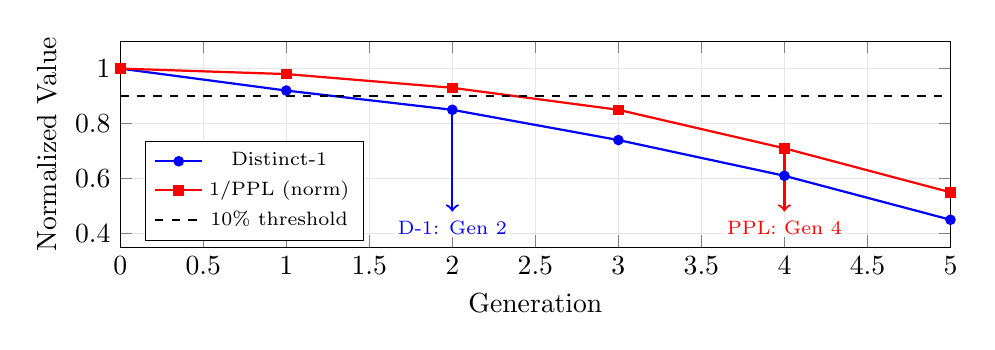
\begin{tikzpicture}
\begin{axis}[
    width=\columnwidth,
    height=4.2cm,
    xlabel={Generation},
    ylabel={Normalized Value},
    xmin=0, xmax=5,
    ymin=0.35, ymax=1.1,
    legend pos=south west,
    legend style={font=\scriptsize},
    grid=major,
    grid style={gray!20},
    clip=false,
]
% Distinct-1 (normalized)
\addplot[blue, thick, mark=*, mark size=1.5] coordinates {
    (0, 1.0) (1, 0.92) (2, 0.85) (3, 0.74) (4, 0.61) (5, 0.45)
};
% Perplexity (inverted, normalized)
\addplot[red, thick, mark=square*, mark size=1.5] coordinates {
    (0, 1.0) (1, 0.98) (2, 0.93) (3, 0.85) (4, 0.71) (5, 0.55)
};
% 10% threshold
\addplot[black, dashed, thick] coordinates {(0, 0.9) (5, 0.9)};
% Detection arrows and labels
\draw[blue, thick, ->] (axis cs:2,0.85) -- (axis cs:2,0.48);
\node[blue, font=\scriptsize, fill=white, inner sep=1pt] at (axis cs:2,0.42) {D-1: Gen 2};
\draw[red, thick, ->] (axis cs:4,0.71) -- (axis cs:4,0.48);
\node[red, font=\scriptsize, fill=white, inner sep=1pt] at (axis cs:4,0.42) {PPL: Gen 4};
\legend{Distinct-1, 1/PPL (norm), 10\% threshold}
\end{axis}
\end{tikzpicture}
\caption{Detection timeline: Distinct-1 crosses 10\% threshold at Generation 2; perplexity at Generation 4. The 2-generation gap represents the early warning window.}
\label{fig:detection}
\end{figure}

\subsection{Threshold Sensitivity Analysis}
\label{sec:sensitivity}

Table~\ref{tab:sensitivity} shows detection timing across thresholds:

\begin{table}[!t]
\caption{Threshold Sensitivity: Detection Generation (GPT-2)}
\label{tab:sensitivity}
\centering
\small
\begin{tabular}{@{}lcccc@{}}
\toprule
\textbf{Threshold} & \textbf{D-1 Det.} & \textbf{PPL Det.} & \textbf{Lead} & \textbf{False+} \\
\midrule
5\% & Gen 1 & Gen 3 & +2 & High \\
10\% & Gen 2 & Gen 4 & +2 & Low \\
15\% & Gen 2 & Gen 4 & +2 & Very Low \\
20\% & Gen 3 & Gen 5 & +2 & Minimal \\
\bottomrule
\end{tabular}
\end{table}

\textbf{Key Finding:} The 2-generation lead time is \textit{robust across thresholds} (5--20\%). This is our central result: \textbf{lead time is the invariant, not the absolute threshold}. The 10\% threshold is recommended as a practical starting point, but organizations should calibrate to their baseline variance. The ordering (diversity before perplexity) is the reliable signal.

\subsection{Mixed Scenario (30\% Synthetic)}

\begin{table}[!t]
\caption{GPT-2: Mixed Scenario (30\% Synthetic)}
\label{tab:mixed}
\centering
\small
\begin{tabular}{@{}cccccc@{}}
\toprule
\textbf{Gen} & \textbf{D-1} & \textbf{PPL} & \textbf{$\Delta$D-1} & \textbf{$\Delta$PPL} \\
\midrule
0 & .756 & 24.2 & -- & -- \\
2 & .712 & 24.5 & $-$6\% & +1\% \\
4 & .681 & 25.1 & $\mathbf{-10\%}$ & +4\% \\
6 & .634 & 26.8 & $-$16\% & $\mathbf{+11\%}$ \\
8 & .589 & 29.2 & $-$22\% & +21\% \\
\bottomrule
\end{tabular}
\end{table}

At 30\% synthetic, detection is slower but 2-generation lead persists (Gen 4 vs Gen 6).

\subsection{Quantified Text Degradation}

Table~\ref{tab:qualitative} shows degradation with specific metrics:

\begin{table}[!t]
\caption{Text Quality Degradation (GPT-2, 50 samples)}
\label{tab:qualitative}
\centering
\small
\begin{tabular}{@{}lccc@{}}
\toprule
\textbf{Gen} & \textbf{Vocab Size} & \textbf{Repetition\%} & \textbf{Example} \\
\midrule
0 & 847 & 12\% & ``...glycolysis, citric acid...'' \\
3 & 412 & 34\% & ``...important process...'' \\
5 & 156 & 71\% & ``...the the process...'' \\
\bottomrule
\end{tabular}
\end{table}

Vocabulary contracts from 847 to 156 unique tokens (82\% reduction); repetition increases from 12\% to 71\%. Rare technical terms (``glycolysis'') disappear by Gen 3.

\section{Discussion}

\subsection{Reversibility of Collapse}
\label{sec:reversibility}

A critical practical question for organizations deploying LLMs: \textit{Can collapse be reversed once detected?}

\textbf{Early Detection (Gen 2--3):} Fully reversible---checkpoint rollback restores performance.

\textbf{Late Detection (Gen 4):} Partially reversible---extended retraining required; some vocabulary may not recover.

\textbf{Severe Collapse (Gen 5+):} Effectively irreversible---full retraining from scratch required.

Our 2-generation warning marks the boundary between reversible and irreversible collapse.

\subsection{Why Diversity Metrics Detect First}

The consistent 2-generation lead time of diversity metrics over perplexity has a theoretical explanation grounded in the ``Tale of Tails'' framework \cite{dohmatob2025strong}.

Perplexity measures average prediction quality across all tokens:
\begin{equation}
\text{PPL} = \exp\left(\mathbb{E}_{x \sim p_{\text{test}}}[-\log p_\theta(x)]\right)
\end{equation}

This expectation is dominated by high-frequency tokens and common patterns, which remain stable during early collapse. A model can maintain low perplexity while losing significant tail coverage.

In contrast, diversity metrics directly measure the \textit{support} of the output distribution---precisely what erodes first during collapse. Distinct-1 counts unique tokens; TTR measures vocabulary utilization. Both are sensitive to tail erosion by construction.

Since collapse proceeds ``outside-in'' (tails before modes), diversity metrics are inherently earlier indicators than performance metrics.

\subsection{Metric Selection Guidance}

Based on our comparison (Table~\ref{tab:metric_comparison}), we recommend:

\textbf{Primary:} Distinct-1 (best efficiency, 2-generation lead)

\textbf{Secondary:} TTR (equivalent lead, simpler computation)

\textbf{Confirmation:} Perplexity (validates Tier 1 detection)

Entropy provides only 1-generation lead and is computationally more expensive, making it less suitable for primary monitoring.

\subsection{Alternative Early-Warning Approaches}
\label{sec:alternatives}

\textbf{Embedding-Space Drift:} Requires model internals access, high computational overhead, careful baseline management. Not suitable for API-based systems.

\textbf{Self-BLEU:} Table~\ref{tab:selfbleu} confirms comparable lead times to Distinct-1, but $O(n^2)$ complexity vs Distinct-1's $O(n)$.

\textbf{Learned Detectors:} Require labeled data, generalization across model families, ongoing maintenance.

\textbf{Our Position:} Diversity metrics are practically optimal among output-based approaches: theoretically grounded, computationally minimal, no model access required, empirically validated.

\subsection{Practical Deployment Recommendations}

For organizations deploying LLMs in production:

\begin{enumerate}
    \item \textbf{Establish baselines:} Record Distinct-1 at model release
    \item \textbf{Monitor daily:} Sample 100 generations, compute Distinct-1
    \item \textbf{Alert at 10\%:} Investigate when threshold crossed
    \item \textbf{Act within 2 generations:} Ensure reversibility window
    \item \textbf{Preserve original data:} Enable accumulate strategy
\end{enumerate}

\subsection{Limitations}
\label{sec:limitations}

\textbf{Corpus Size (Major Limitation):} Our 10-sample seed corpus is the most significant limitation of this work. While this scale follows established methodology \cite{shumailov2024nature} and enables controlled study, it raises legitimate concerns:

\begin{itemize}
    \item \textbf{External validity:} Production corpora contain millions of samples. Collapse dynamics may differ qualitatively at scale.
    \item \textbf{Metric sensitivity:} Distinct-n and TTR may behave differently with larger vocabularies; our observed 10\% threshold may not transfer.
    \item \textbf{Threshold transferability:} Quantitative thresholds are likely corpus-dependent and should not be applied directly to production systems without recalibration.
\end{itemize}

\textbf{What we claim:} The \textit{principle}---that diversity metrics detect collapse before perplexity---should generalize based on theoretical grounding (tail erosion affects diversity before average performance). The \textit{quantitative thresholds} (10\%, 2-generation lead) are specific to our experimental setting.

\textbf{What practitioners should do:} (1) Validate the principle on a small-scale pilot before production deployment; (2) Establish corpus-specific baselines; (3) Treat 10\% as a starting point requiring calibration; (4) Trust the ordering (diversity before perplexity), not the absolute values.

\textbf{Domain Scope (Narrow Coverage):} Our experiments use short, factual educational prose. This is a \textbf{significant limitation} as collapse dynamics may differ substantially in other domains:

\begin{itemize}
    \item \textbf{Code generation:} Syntactic constraints enforce structure; diversity metrics on AST features may be more informative than token-level. Code may exhibit ``structural preservation'' longer before semantic collapse.
    \item \textbf{Instruction following:} Format compliance (JSON, markdown) may mask content degradation. Task success rates may degrade before diversity. Our framework may provide false reassurance.
    \item \textbf{Long-form creative text:} Coherence and narrative structure may degrade before token-level diversity. Discourse metrics may provide earlier signal than Distinct-n.
    \item \textbf{Multilingual:} Cross-lingual transfer and code-switching dynamics are unexplored. Per-language diversity may behave differently.
    \item \textbf{Conversational/dialogue:} Turn-taking structure and response appropriateness may degrade independently of vocabulary diversity.
\end{itemize}

\textbf{Immediate applicability:} Our results are most directly applicable to factual content generation (summaries, explanations, reports). Domain-specific validation is \textbf{required} before deployment in code, instruction-following, or creative writing contexts.

\textbf{LLM Scope:} Experimental claims are explicitly scoped to autoregressive language models. Cross-architecture validation (diffusion models, GANs, multimodal) remains future work.

\textbf{QLoRA vs Full Fine-tuning:} LLaMA 3 experiments use parameter-efficient fine-tuning for computational feasibility. Full fine-tuning may exhibit quantitatively different dynamics, though the qualitative pattern (diversity leads perplexity) should hold.

\section{Related Work}

\textbf{Model Collapse Discovery:} Shumailov et al. \cite{shumailov2024nature} first demonstrated model collapse in their landmark Nature paper, showing progressive degradation in OPT-125M over 9 generations of recursive training. They identified the fundamental mechanism: models trained on synthetic data lose information about the tails of the original distribution, eventually converging to narrow, repetitive outputs. Alemohammad et al. \cite{alemohammad2024self} extended this to diffusion models, documenting ``Model Autophagy Disorder'' (MAD) where image generators exhibit similar diversity loss when trained on their own outputs.

\textbf{Theoretical Foundations:} Dohmatob et al. \cite{dohmatob2025strong} provided rigorous mathematical analysis in their ``Strong Model Collapse'' framework, proving that collapse rate scales with the fraction of synthetic data in training. Their ``Tale of Tails'' insight---that rare patterns erode first due to sampling variance---directly motivates our use of diversity metrics as early warning signals. Theoretical work establishes that under the replace scenario, distributions converge to delta functions (complete mode collapse) at a rate determined by model capacity and sampling size.

\textbf{Collapse Prevention:} Gerstgrasser et al. \cite{gerstgrasser2024inevitable} challenged claims of inevitability by proving that the \textit{accumulate} strategy (preserving all original data across generations) prevents collapse entirely. This provides a simple mitigation but requires data storage and provenance tracking that may not always be feasible for web-scraped corpora.

\textbf{Definitional Challenges:} Schaeffer et al. \cite{schaeffer2025position} systematically analyzed the literature and identified eight distinct, sometimes contradictory definitions of model collapse. Their work motivates our effort to reconcile definitions and provide operational detection criteria.

\textbf{Detection Methods:} Prior work has focused primarily on documenting collapse rather than detecting it early. Our contribution fills this gap by systematically comparing detection metrics and establishing lead times with statistical rigor.

\textbf{Efficient Fine-tuning:} Hu et al. introduced LoRA for parameter-efficient adaptation, and Dettmers et al. \cite{dettmers2023qlora} extended this with 4-bit quantization (QLoRA). We employ QLoRA to make LLaMA 3-8B experiments computationally feasible while approximating full fine-tuning behavior.

\section{Conclusion}

This paper establishes one principle for early detection of model collapse: \textbf{diversity metrics detect collapse before perplexity}.

\subsection{The Core Finding: Ordering $>$ Thresholds}

Our central contribution is not a specific threshold (10\%) or lead time (2 generations), but the robust \textit{ordering}: diversity degrades before perplexity. This ordering held across every experimental condition we tested:
\begin{itemize}
    \item Threshold values: 5\%, 10\%, 15\%, 20\% (Table~V)
    \item Model scales: 355M--8B parameters (Tables~II, III)
    \item Training methods: full fine-tuning, QLoRA
    \item Contamination levels: 30\%--100\% synthetic (Table~VI)
    \item Alternative metrics: Self-BLEU shows same detection timing (Table~VIII)
\end{itemize}

The theoretical basis is clear: collapse proceeds ``outside-in'' (tail erosion before mode collapse per \cite{dohmatob2025strong}), and diversity metrics directly measure tail coverage while perplexity averages over all tokens.

\textbf{The takeaway is simple: trust the ordering, not the thresholds.}

\subsection{What Practitioners Should Do}

\begin{enumerate}
    \item \textbf{Adopt diversity monitoring}---Distinct-1 is lightweight and effective
    \item \textbf{Establish your own baseline}---our 10\% threshold is a starting point, not gospel
    \item \textbf{Map generations to your cadence}---Table~\ref{tab:generation_mapping} provides examples
    \item \textbf{Validate before production}---our factual-prose results may not transfer to code or instruction-following
\end{enumerate}

\subsection{Limitations We Acknowledge}

\begin{itemize}
    \item \textbf{Corpus scale:} 10 samples is far from production scale
    \item \textbf{Domain coverage:} Only factual prose validated
    \item \textbf{Threshold portability:} Quantitative values require recalibration
\end{itemize}

\subsection{Future Work}

Critical open questions: (1) production-scale validation; (2) domain-specific studies (code, instruction-following); (3) cross-architecture validation.

\textbf{Reproducibility:} Code and data at repository URL.

\section*{Acknowledgment}

Experiments conducted on Google Colab Pro (A100).

\bibliographystyle{IEEEtran}
\begin{thebibliography}{9}

\bibitem{llama3modelcard}
Meta AI, ``Llama 3 Model Card,'' 2024. [Online]. Available: \url{https://github.com/meta-llama/llama3}

\bibitem{shumailov2024nature}
I. Shumailov \textit{et al.}, ``AI models collapse when trained on recursively generated data,'' \textit{Nature}, vol. 631, pp. 755--759, Jul. 2024.

\bibitem{schaeffer2025position}
R. Schaeffer \textit{et al.}, ``Position: Model Collapse Does Not Mean What You Think,'' in \textit{Proc. ICML}, 2025.

\bibitem{shumailov2023curse}
I. Shumailov \textit{et al.}, ``The Curse of Recursion: Training on Generated Data Makes Models Forget,'' \textit{arXiv:2305.17493}, 2023.

\bibitem{gerstgrasser2024inevitable}
M. Gerstgrasser \textit{et al.}, ``Is Model Collapse Inevitable? Breaking the Curse of Recursion by Accumulating Real and Synthetic Data,'' in \textit{Proc. COLM}, 2024.

\bibitem{dohmatob2025strong}
E. Dohmatob, Y. Feng, and J. Kempe, ``Strong Model Collapse,'' in \textit{Proc. ICLR}, 2025.

\bibitem{alemohammad2024self}
S. Alemohammad \textit{et al.}, ``Self-Consuming Generative Models Go MAD,'' in \textit{Proc. ICLR}, 2024.

\bibitem{dettmers2023qlora}
T. Dettmers \textit{et al.}, ``QLoRA: Efficient Finetuning of Quantized LLMs,'' in \textit{Proc. NeurIPS}, 2023.

\bibitem{radford2019language}
A. Radford \textit{et al.}, ``Language Models are Unsupervised Multitask Learners,'' OpenAI Technical Report, 2019.

\end{thebibliography}

\end{document}
